\chapter{Hito 6 - Evaluación heurística}
Uno de los puntos más importantes del proceso de Diseño Guiado por Objetivos es la evaluación de la usabilidad de los
prototipos que han sido desarrollados en la etapa del Framework. Existen varios métodos a través de los cuales es posible
obtener una evaluación completa, pero en nuestro caso nos vamos a centrar en las evaluaciones heurísticas, ya que nos van a poner
proporcionar los principales problemas que tiene nuestra interfaz referente a la usabilidad. \\

Hemos optado por realizar en primer lugar una evaluación heurística antes que una evaluación con usuarios debido al coste
que supone esta última, de modo que así podremos minimizar el coste que supondría en la siguiente fase de la evaluación (ya realizaremos
una evaluación con los usuarios finales de nuestra aplicación). \\

Por tanto, el objetivo que vamos a tener en este hito va a ser realizar sesiones de evaluación de nuestra aplicación en las que los miembros
de nuestro equipo van a actuar como experimentadores y los miembros de grupo 6 como expertos que van a evaluar el prototipo con las heurísticas
proporcionadas para hacernos una idea de los principales fallos que pueden identificarse. En cuanto a las tareas que se han realizado, hemos hecho
las siguientes en el orden que se expresa:
\begin{enumerate}
    \item \textbf{Selección de la heurística} $\rightarrow$ vamos a realizar una reunión inicial de planificación en la que van a tomarse las principales
    decisiones acerca de las sesiones de evaluación, como va a ser el caso de la decisión de la heurística con la que los expertos del otro grupo van a evaluar
    nuestro prototipo.
    \item \textbf{Preparación de la sesión} $\rightarrow$ el otro de los puntos que se va a tratar en la sesión inicial va a ser preparar la sesión de evaluación,
    es decir, ver el material que van a proporcionar los experimentadores a los expertos del otro grupo para poder realizar una correcta evaluación, así como la
    redacción del guión de actividades que van a tener que seguir para obtener la valoración buscada.
    \item \textbf{Sesiones de evaluación} $\rightarrow$ en ellas es donde realmente se va a realizar la evaluación definitiva de nuestro prototipo. Nuestro grupo se va
    a dividir en dos: 5 de nuestros miembtos actuarán como expertos y valorarán el prototipo del otro grupo, mientras que los otros 5 participarán como experimentadores
    que guiarán a los expertos del otro grupo para que puedan evaluar el prototipo con las heurísticas que les hemos proporcionado.
    \item \textbf{Debriefing} $\rightarrow$ tras haber finalizado las sesiones de evaluación, es necesario dejar un tiempo de descanso y posteriormente realizar una sesión de
    debriefing, en las que se realizará una puesta en común de todo lo que se ha observado y obtenido en las sesiones de evaluación, para poder discutir cómo puede ser solucionado y
    asignarle así una prioridad a cada uno de los problemas que se han identificado.
    \item \textbf{Evaluación del trabajo realizado por otros expertos} $\rightarrow$ se evalúa de forma justificada el trabajo realizado por cada uno de los expertos del otro grupo de forma individual.
    Además se va a indicar lo que se hizó bien, qué se hizó mal y la calidad de la evaluación realizada por cada uno de los expertos.
    \item \textbf{Evaluación de las sesiones de evaluación realizadas para otro grupo} $\rightarrow$ los expertos de nuestro equipo van a evaluar cómo han realizado las distintas sesiones
    del otro grupo, el material que se les ha proporcionado para la evaluación y algunos de los problemas que se han encontrado.
    \item \textbf{Cambios en el prototipo} $\rightarrow$ tras haber realizado una valoración de los problemas que se han obtenido y ordenados por prioridad, vamos a realizar las modificaciones
    necesarias en el prototipo de Figma para dejarlo listo para la evaluación con usuarios.
\end{enumerate}

\section{Planificación}
Con la finalidad de poder organizarnos para el transcurso de este hito, hemos tenido que listar las distintas tareas que van a realizarse (las ya descritas en la introducción) y se ha asignado a 
cada uno de los miembros. El tiempo para el que se ha planificado ha sido la semana del 11 de diciembre y lo planificado para los días 11 y 13 (la reunión de preparación y la de las sesiones de evaluación)
se han realizado en las sesiones de laboratorio de esos días. En la figura \ref{fig:planif-h6} se puede observar el diagrama de la planificación.
\begin{figure}
    \centering
    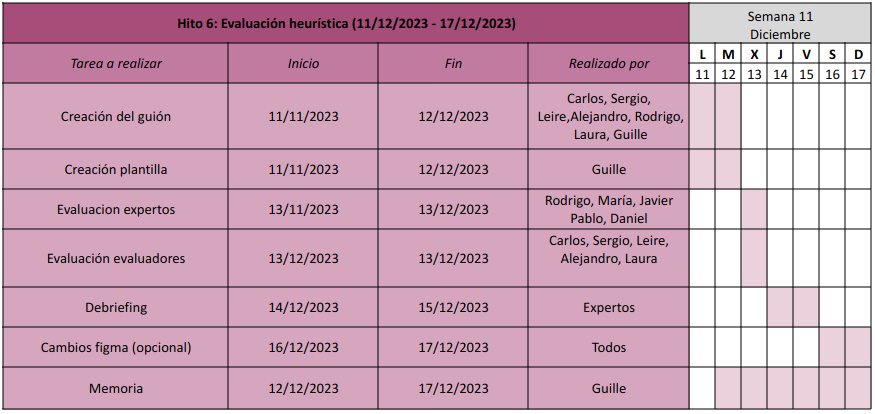
\includegraphics[width=1\textwidth]{Imagenes/Planificaciones/Planif-hito6.png}
    \caption{Planificación Hito 6}
    \label{fig:planif-h6}
\end{figure}

\section{Selección de la heurística}
Como ya mencionamos anteriormente, realizamos una reunión inicial el lunes 11 en el laboratotio de clase para poder planificar las sesiones de evaluación que iban a llevarse a cabo. Uno de los puntos que fue tratado
en esta reunión fue la selección de la heurística que iban a utilizar los expertos para poder evaluar y extraer los principales problemas de nuestro prototipo. En cuanto a las opciones barajadas, fueron las siguientes:
\begin{itemize}
    \item \textbf{10 principios de diseño de Nielsen} $\rightarrow$ surgen tras un estudio de cómo poder mejorar la interacción entre el humano y el ordenador. Actualmente se
    siguen tomando como medida para medir la usabilidad e identificar errores.
    \item \textbf{8 reglas de oro de Shneiderman} $\rightarrow$ son principios de diseño de interfaces de usuarui que se centran en mejorar la usabilidad y la experiencia
    del usuario. Proporcionan pautas valiosas para diseñadores y desarrolladores de software.
    \item \textbf{Principios heurísticos de Larry Constantine} $\rightarrow$ propone una serie de principios para conseguir una interfaz usable y se basa en varios conceptos, como
    la estructura, la simplicidad o la visibilidad.
    \item \textbf{Principios heurísticos de Keith Instone} $\rightarrow$ relata una serie de principios básicos que han de tenerse en cuenta al desarrollar una interfaz.
\end{itemize}

Finalmente, tras haber planteado estas opciones entre las heurísticas que se iban a utilizar, hemos optado por emplear los 10 principios de diseño de Nielsen, ya que se siguen
usando hoy en día para mejorar la interacción del usuario con la aplicación y la usabilidad. Entre algunos de los motivos por los que hemos decidido esta heurística, tenemos el
enfoque en el usuario, ya que prioriza la experiencia del usuario sobre el diseño interno del sistema y la consistencia en el diseño, ya que ayuda a los usuarios a sentirse cómodos
al interactuar con el prototipo que hemos diseñado.

\section{Preparación de la sesión}
Tras haber seleccionado la heurística que se iba a utilizar en nuestra evaluación, el siguiente punto de la reunión que fue tratado fue la preparación de la sesión. Esta preparación consistió en recopilar
el material que los experimentadores iban a entregar a los expertos, así como la redacción del guión de actividades que debían ser evaluadas con las heurísticas anteriormente seleccionadas. Vamos a centrarnos
en primer lugar en este guión de actividades. \\

Para poder conformarlo, se han tomado distintas actividades, tanto propuestas por nosotros, como otras presentes tanto en los escenarios keypath como en los escenarios de validación del hito anterior. Estas actividades
son las siguientes:
\begin{enumerate}
    \item Filtrar los viajes por tipo de transporte.
    \item Registrarse e iniciar sesión.
    \item Cerrar sesión.
    \item Ver detalles de los viajes.
    \item Consultar un viaje accesible sin ser un usuario con discapacidad.
    \item Consultar los datos de una reserva y descargar los billetes.
    \item Ordenar los resultados del comparador por precio de menor a mayor.
    \item Comprobar los datos de una reserva.
    \item Consultar en preguntas frecuentes ¿Cómo modificar mi reserva?
    \item Solicitar ayuda en el soporte electrónico del chat.
    \item Comprar billetes para una ciudad con comida y cama.
    \item Cancelar un viaje.
    \item Modificar el DNI del usuario.
    \item Filtrar los viajes por un precio menor de 50€.
    \item Mostrar sólo los viajes directos (sin escalas), escoger uno y reservarlo pagando con
    tarjeta.
    \item Hacer una búsqueda con intervalo de tiempo de un mes y para dos personas.
    \item Mostrar únicamente los trenes en la búsqueda.
    \item Entrar al perfil y volver.
    \item Modificar los datos de una reserva.
    \item Anular a un acompañante.
\end{enumerate}

Acompañado a este guión de actividades, se propuso una breve presentación de la aplicación, que incluía las funcionalidades que se habían abarcado, así como una breve descripción del entorno de
la aplicación, para posteriormente dejar al usuario la libertad de interactuar con ella antes de comenzar la sesión. Tras haber readactado este guión que debe de seguir el experto para evaluar las
heurísticas, se ha preparado también material adicional que iba a servir de referencia para el usuario. \\

El primero de ellos era una plantilla de acta que los experimentadores de nuestro grupo iban a rellenar en la sesión de evaluación, anotando todos los problemas y el comportamiento del experto
durante el transcurso de la sesión. La estructura de esta plantilla se puede ver en la figura \ref{fig:pla-actases}. Como se puede ver, el contenido que tiene es la fecha en la que tuvo lugar la sesión,
los participantes (el experto y el experimentador), las anotaciones del desarrollo de la sesión y una serie de conclusiones finales. En cuanto al prototipo empleado, se trata
del mismo que el hito anterior sin modificaciones realizadas, que puede verse \href{https://www.figma.com/file/YGz2UUMhvxNOTCHhu1TZle/Just-Travel-It?type=design&node-id=0%3A1&mode=design&t=18R6j8wE0vfjz3qF-1}{aquí}.
\begin{figure}[h]
    \centering
    \includegraphics[width=0.6\textwidth]{Imagenes/Hito6/Acta de Sesión.png}
    \caption{Plantilla del Acta de Sesión}
    \label{fig:pla-actases}
\end{figure}

En cuanto a la documentación proporcionada a los expertos, tenemos un listado con la heurística que ha de emplearse (para que puedan consultarla fácilmente en cualquier momento), así como una plantilla en Excel
con todas las actividades y un listado de apartados a rellenar en caso de que el usuario experto haya detectado alguna violación de las heurísticas mencionadas. En cuanto al contenido de la misma, podemos 
encontrar la heurística que se ha violado, una descripción del problema, el lugar del prototipo en el que se puede encontrar el fallo, el motivo de la violación y la severidad. Además, el contenido se encuentra
claramente dividido por actividades. En la figura \ref{fig:pla-exp} podemos ver un fragmento de esta plantilla a modo de ejemplo. \\

Por último, y para finalizar la sesión, se decidieron los roles que iba a tener cada uno de los miembros del grupo en las sesiones de evaluación. Cabe destacar que al ser 11 miembros, uno de nosotros, como ya se puede
ver en la planificación, se ha encargado de la redacción de la memoria y supervisión de las sesiones de evaluación de nuestros examinadores. Finalmente, la adjudicación de roles quedó así:
\begin{itemize}
    \item \textbf{Expertos} $\rightarrow$ Rodrigo, María, Daniel, Pablo y Javier.
    \item \textbf{Experimentadores} $\rightarrow$ Leire, Sergio, Alejandro, Carlos y Laura.
    \item \textbf{Memoria y supervisión} $\rightarrow$ Guillermo
\end{itemize}

\begin{figure}[h]
    \centering
    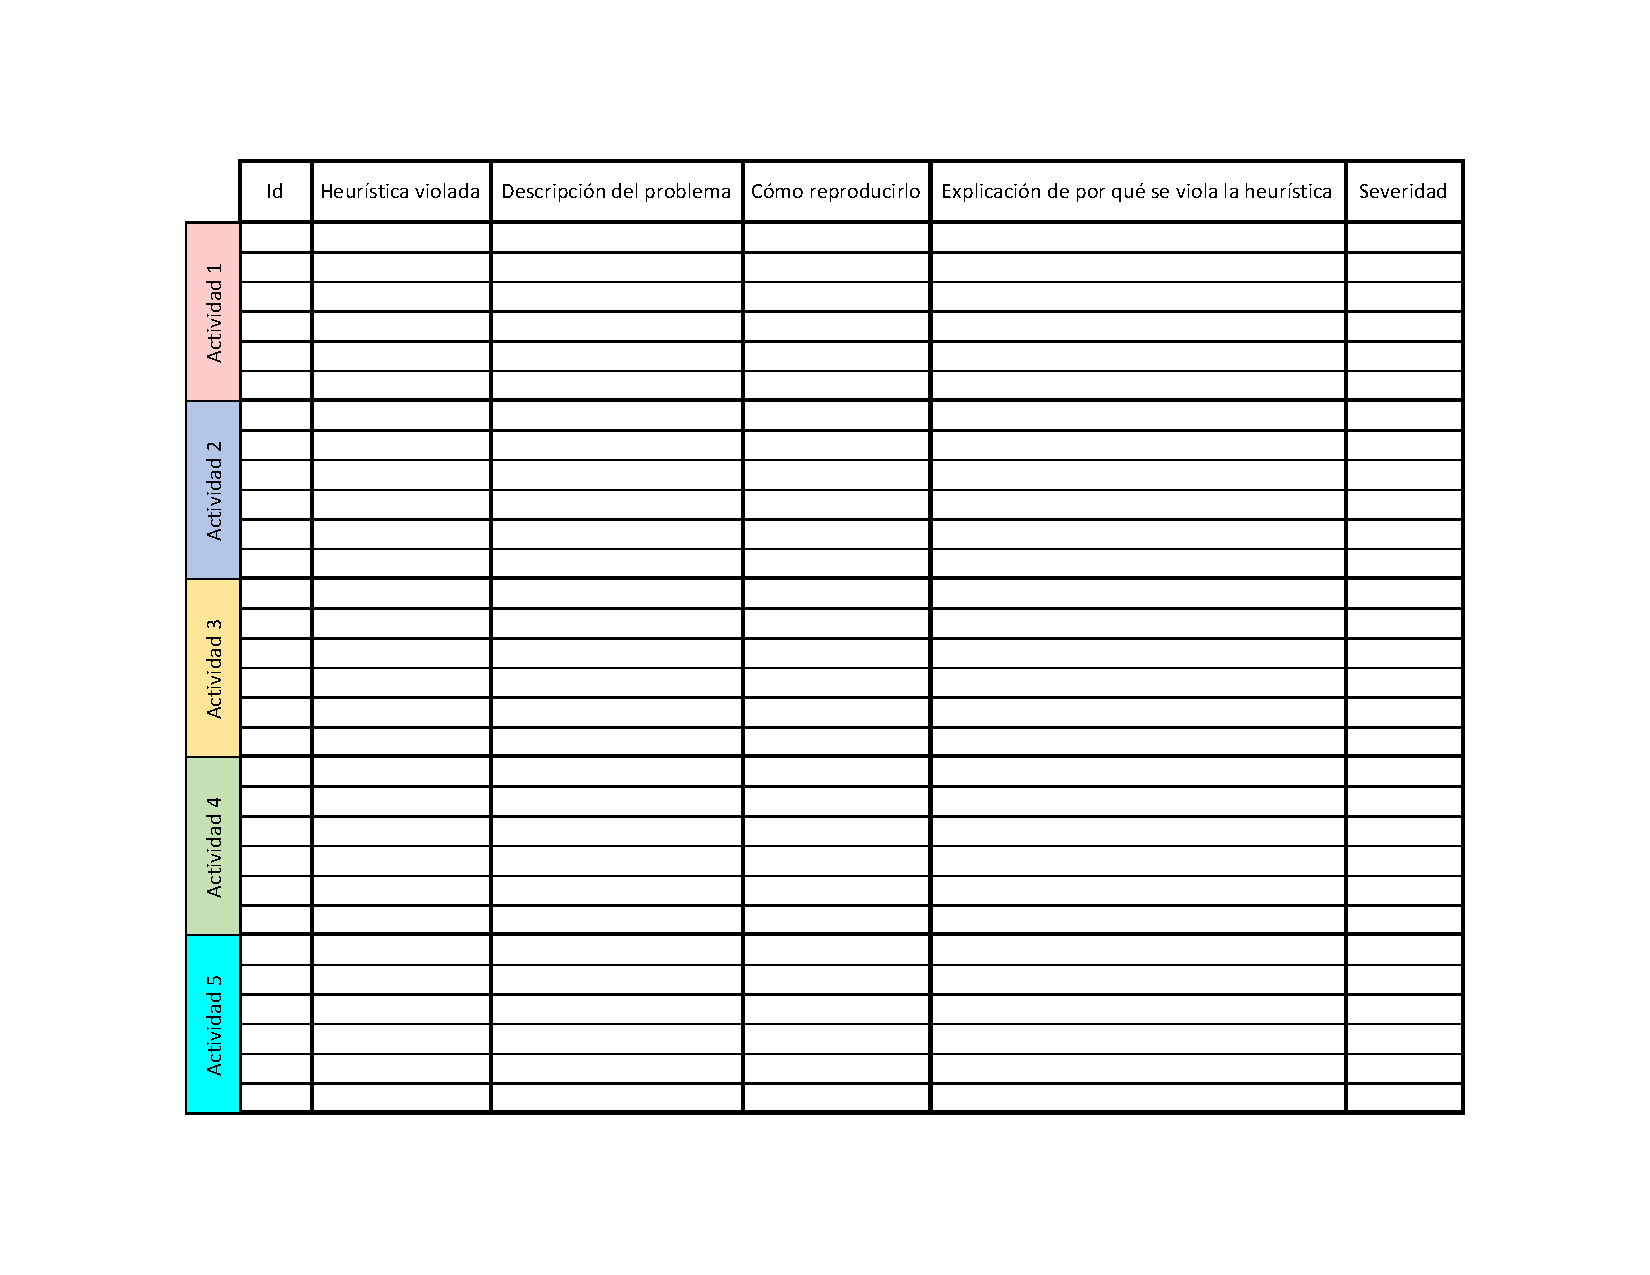
\includegraphics[width=1\textwidth]{Imagenes/Hito6/PlantillaEval.pdf}
    \caption{Plantilla de Evaluación Expertos}
    \label{fig:pla-exp}
\end{figure}

\section{Sesiones de evaluación}
Una vez recopilado todo el material necesario, definidos los roles y planificado cómo se va a realizar la sesión de evaluación, el miércoles 13 tuvieron lugar las mismas en la sesión de laboratorio. El funcionamiento fue el siguiente:
los experimentadores de nuestro equipo recibieron a los expertos del otro equipo y les describieron la idea principal que iba a tener el proyecto, así como las distintas actividades que debían replicar y las
heurísticas con las que tenían que hacerlo. Por otro lado, los expertos designados por nuestro equipo se sentaron con los experimentadores del otro equipo para poder realizar la evaluación de su aplicación (los
roles seguidos se encuentran detallados en la sección anterior). \\

El material proporcionado a cada uno de los expertos del grupo 6 puede ser consultado y se trata de un enlace al prototipo en Figma que debe ser evaluado, un listado de las distintas actividades que han de probarse
(para tenerlas a mano), otro listado con las heurísticas que hemos elegido para también tenerlas a mano y una plantilla en la que poder rellenar con aquellos problemas que se han identificado en el prototipo debido
a posibles violaciones de las heurísticas. \footnote{\href{https://drive.google.com/drive/folders/1WBsmnExJs_6jhmdTfktGOwBWZRp-Su1W?usp=drive_link}{Enlace al material proporcionado}} Cabe destacar también que
durante el transcurso de las diferentes sesiones, los expertos no han hablado entre sí y en cada una de las sesiones había un experto y un experimentador. Al comenzar cada una de las sesiones, se presenta al usuario experto
la aplicación, indicando las funcionalidades que abarca, así como posteriormente otorgarle libertad para familiarizarse con la aplicación. \\

Cabe destacar además que la severidad de los problemas identificados fue asignada por el experto al finalizar todas las atividades planteadas y encontrados todos los problemas. En este apartado nos centraremos en el transcurso de las sesiones de evaluación que fueron realizadas a nuestro equipo por parte de los expertos del grupo 6. Como ya hemos descrito anteriormente, el producto de
cada una de las sesiones va a ser un acta de la sesión, redactada por nuestro experimentador informando acerca de los problemas identificados en la sesión y los comentarios adicionales que ha podido realizar el
experto del otro equipo, así como también un listado de los problemas que se han encontrado en el prototipo debido a violaciones de las heurísticas que habíamos seleccionado como método de evaluación. Veamos ahora
en detalle cada una de las cinco sesiones de evaluación que tuvo lugar:
\subsection{Sesión 1 - Experimentador Carlos}
\subsubsection{Acta de la sesión de evaluación - Carlos - 13/12/2023}
\subsubsection{Participantes}
\begin{itemize}
    \item \textit{Experimentador} $\rightarrow$ Carlos Varela Sansano
    \item \textit{Experto} $\rightarrow$ Jaime Costas Insúa
\end{itemize}

\subsubsection{Desarrollo de la sesión}\label{sec:sesiones}
\begin{itemize}
    \item Le parece inconsistente que los filtros de transporte estén encima (al filtrar por transporte) y no a la izquierda con el resto de filtros, 
    viola la heurística n"o 4.
    \item Le parece que al registrarse no hay mensaje de confirmación y no queda claro que estás logueado en la aplicación, violando así la heurística n"o 1.
    \item Cerrar sesión le parece que está bien.
    \item Ver detalles de los viajes está bien. 
    \item Buscar viajes accesibles no mantiene una consistencia porque el checkbox actúa como un botón y no tiene esa función, también ocurre que no está en todas las 
    pantallas de buscar la opción de viaje accesible. 
    \item No se pueden consultar los datos de ninguna reserva, ya que no hay flujo que llegue hasta ahí. También dice que hay demasiados datos innecesarios.
    \item No se puede consultar los datos de ninguna reserva.
    \item El botón de ver preguntas frecuentes es muy pequeño, violando la heurística n"o 10 de ayuda y documentación.
    \item El botón de soporte es muy pequeño, violando la heurística n"o 10 de ayuda y documentación. Mensaje automático de que se responderá pronto.
    \item Comprar billete con comida y cama no aparece luego en el resumen de comprar billete, no mantiene la consistencia. Coger cama en una avión le parece raro.
    \item Cancelar viaje no lleva a ningún lado, el resto está bien.
    \item Modificar datos del usuario muy intuitivo.
    \item Pedimos filtrar por menos de 50€ y sale por menos de 25€. No mantiene la consistencia y estándares. No se puede mover la barra (pero es imposible 
    mover el puntero en la barra).
    \item Filtrar por viajes directos al principio no es buena opción. Debería estar seleccionado sin escalas al inicio. El resto bien. 
    \item Poner la fecha en el desplegable no funciona, escoger número de personas bien. Lo único que no hemos metido ninguna pantalla de carga. 
    \item No se pueden modificar los trenes, sólo los vuelos.
    \item Entrar al perfil y volver bien. 
    \item Modificar datos del usuario se debería llamar de otra forma para no llevar a errores.
    \item El botón de cancelar la reserva no está claro, ya que parece que vas a cancelar toda la reserva y no solo un billete. 
\end{itemize}


\subsubsection{Conclusiones finales}
Jaime ha comenzado a interactuar con la aplicación para familiarizarse. Tras la sesión hemos comentado los problemas que han surgido 
a la hora de realizar las tareas, y le ha dado un grado de severidad, también ha sugerido cambios para mejorar el prototipo, como por ejemplo hacer los botones de 
chat y de preguntas frecuentes hacerlos más grandes, Los filtros de transporte nos ha propuesto ponerlos a la izquierda en vez de a la derecha. El botón de viaje 
accesible no aparece en todas las pantallas en vez de ser un checkbox funciona como un botón. para cancelar un billete solo en vez de todo el viaje no queda claro 
cómo hacerlo. No le gustó que en un avión se pudiese escoger la opción de cama, en vez de eso propone poder coger billetes business. Dice que no queda claro que 
poner una imagen genérica a la hora de iniciar sesión, no demuestra que este la sesión iniciada, propone un mensaje de éxito al iniciar sesión. También nos ha dicho 
que no tenemos pantalla de carga entre pantallas, dice que sería conveniente meterlas en las pantallas de pago.

\subsection{Sesión 2 - Experimentador Alejandro}
\subsubsection{Acta de la sesión de evaluación - Alejandro - 13/12/2023}
\subsubsection{Participantes}
\begin{itemize}
    \item \textit{Experimentador} $\rightarrow$ Alejandro Barrachina Argudo
    \item \textit{Experto} $\rightarrow$ Miguel de Areba
\end{itemize}

\subsubsection{Desarrollo de la sesión}
El planteamiento de las anotaciones que se han realizado viene dado por la actividad, de modo que para cada una de las actividades se han realizado las anotaciones pertinentes.
\begin{enumerate}
    \item El experto consigue buscar un viaje. El usuario tiene problemas  a la hora del ordenado ya que no le deja escoger un tipo de transporte tras ordenar (posible limitación de figma). El experto esperaba el filtro de transportes dentro del apartado de filtros.
    \item No se pueden rellenar datos en el figma. El usuario consigue registrarse e iniciar sesión.
    \item El usuario consigue cerrar sesión.
    \item El usuario no ve de primeras el botón de detalles. El usuario sugiere cambiar el color del botón.
    \item El usuario no ve diferencia al no ver el icono. El color verde resalta.
    \item No funciona en el figma para ver los datos de reservas. El usuario puede consultar los detalles del viaje pero no descargar los billetes. El usuario tenía intención de usar el “botón del ojo”. Se sugiere otro botón directo de descarga.
    \item El usuario la hace rápido.
    \item Misma que la 6 sin la parte de descarga.
    \item El usuario sugiere aumentar el tamaño de los botones de la esquina, se ven chiquitos.
    \item El usuario consigue escribir un mensaje al soporte.
    \item El usuario sugiere cambiar el espacio entre separadores, se encuentra bien los datos adicionales.
    \item Botón de cancelar roto, El usuario llega hasta la página de reservas.
    \item No se puede cambiar el dni, llega a la ventana de modificar datos.
    \item El usuario filtra rápido y bien.
    \item El usuario no ve la opción de viaje directo, el filtro tampoco cambia nada. El filtrado por vuelos hace que la pantalla no interactúe. El pago se hace bien.
    \item El usuario usa bien el calendario.
    \item No funciona el botón, pero el usuario sabe qué botón usar.
    \item Lo hace bien, ya lo ha hecho en las anteriores actividades.
    \item El usuario dice que es intuitivo, lo hace bastante rápido.
    \item El usuario de primeras intenta hacerlo en  “modificar el billete”. luego va a la página de mis reservas. Tras seleccionar los usuarios no se puede dar a confirmar. El usuario espera cancelar todo el viaje con el botón de cancelar, y modificar los viajeros en modificar viaje
\end{enumerate}


\subsubsection{Conclusiones finales}
El usuario dice que en general la página es bastante intuitiva, lo único que le choca son los colores, todo muy azul y pobre distinción. El perfil le ha parecido de 
lo mejor de la aplicación, muy limpio y con la información necesaria, muy intuitiva. La búsqueda de viaje le parece caótica, le parece cómodo tener ida y vuelta de 
forma contigua. El resumen le parece bien como retroalimentación, seguir explorando podría llevar al comparador de vuelta.

\subsection{Sesión 3 - Experimentador Laura}
\subsubsection{Acta de la sesión de evaluación - Laura - 13/12/2023}
\subsubsection{Participantes}
\begin{itemize}
    \item \textit{Experimentador} $\rightarrow$ Laura Martínez Tomás
    \item \textit{Experto} $\rightarrow$ Christian Sawadogo
\end{itemize}

\subsubsection{Desarrollo de la sesión}
El planteamiento de las anotaciones que se han realizado viene dado por la actividad, de modo que para cada una de las actividades se han realizado las anotaciones pertinentes.
\begin{enumerate}
    \item Ha tenido problemas para buscar los tipos de transporte, ha ido directo a los filtros de la parte derecha por intuición.
    \item No ha tenido problemas para encontrar el botón de registro e inicio de sesión, lo ha visto simple y muy parecido al resto. Pero ve problemas para volver atrás porque la cruz no es muy normal para volver atrás.Y necesita iconos en registro porque hay demasiada información y la gente se puede distraer y no atender (sobre todo veo el problema para gente con discapacidad). Al iniciar sesión echa en falta la opción de olvidó contraseña para cuando se le olvida esta.
    \item Le parece intuitivo cerrar sesión, no ha tenido problema al encontrarlo.
    \item Ha tenido problemas para encontrarlo porque el icono de información es muy pequeño y no le parece intuitivo. Él ha hecho clic en el viaje pensando que le mostraría la información del viaje y por eso le ha costado ver que tenía que dar en el botón de información. Un cambio que le parece bien es que al seleccionar te aparezca la información y un botón debajo de seleccionar o no el viaje.
    \item La casilla de viaje accesible es muy pequeña para ver en el buscador y no tiene sentido que haya dos veces el botón de viaje accesible para gente sin discapacidad.
    \item Está teniendo problemas para saber dónde están los datos de la reserva. El botón del ojo no se entiende que es para eso y además de que están muy pegados los botones a la derecha.
    \item Está bien la opción de ordenar.
    \item No se han identificado problemas.
    \item Muy pequeño el botón y la posición de los botones deberían estar en la misma posición. Está la página de preguntas frecuentes.
    \item Los mismos problemas que los de la tarea 9
    \item Sería mejor separar los servicios porque están en el mismo para ida y vuelta y no tiene sentido porque puedes querer solo de uno. Y sería mejor separar todos los pasos: escoger viaje ida > rellenar información de viajero 1 > viajero 2 > viajero X > servicios y asientos > escoger viaje vuelta > viajeros 
    \item No es intuitivo, deberías seleccionar y que te marque la reserva que quieres eliminar y entonces te aparezcan las opciones. Mismos problemas que los de la tarea 6. Y además si solo quieres cancelar la ida es un problema porque cancelas todo.
    \item Muy fácil e intuitivo.
    \item La sección de filtros debería ser más pequeña, hay mucho espacio y quita al comparador espacio. Pero es fácil de usar.
    \item Los mismos problemas que los de la tarea 11, el resumen de la reserva al final donde el pago está bien, pero lo anterior no. Cuando ya has comprado el mensaje que aparece debería estar más destacado porque es importante saber que se ha hecho todo correctamente.
    \item Mismos problemas que los de la tarea 14.
    \item Está bien.
    \item No se ha detectado ningún problema.
    \item Tienen los mismos problemas que los de las tareas 11 y 12.
    \item Está bien. 
\end{enumerate}


\subsubsection{Conclusiones finales}
Hay que corregir la interfaz de la aplicación para facilitar su uso y que sea más intuitiva ya que el experto ha tenido problemas para 
poder realizar muchas tareas. Además que la gente con ciertas discapacidades tendrán problemas para usarla. \\

El diseño también se tiene que cambiar con las correcciones dichas ya que hay muchos errores referentes a este, como el diseño de los botones de modificar, eliminar 
y consultar en mis reservas. \\

Finalmente, hay muchos problemas de heurísticas por lo que la interfaz no está muy bien diseñada porque en más de la mitad de las tareas se ha detectado más de dos 
heurísticas incumplidas. La mayoría de las heurísticas incumplidas han sido la número 4 y 8 que son referentes a la consistencia (tanto externa como interna) y a 
la estética.

\subsection{Sesión 4 - Experimentador Sergio}
\subsubsection{Acta de la sesión de evaluación - Sergio - 13/12/2023}
\subsubsection{Participantes}
\begin{itemize}
    \item \textit{Experimentador} $\rightarrow$ Sergio Colet García
    \item \textit{Experto} $\rightarrow$ Ismael Barahona
\end{itemize}

\subsubsection{Desarrollo de la sesión}
A lo largo de la evaluación han habido bastantes problemas con respecto al uso del prototipo de Figma, debido a que faltaban algunas de las funcionalidades que 
eran necesarias para hacer todas las tareas. Intentamos arreglarlas antes pero no nos dio tiempo y faltaron varias. \\

Hicimos 2 iteraciones de las tareas, una inicial en la que el experto apuntó los fallos más evidentes del diseño y una segunda para apuntar los que se le habían 
podido escapar. Tras esto, procedió a la evaluación de la severidad de cada uno de los problemas. \\

Durante la sesión apenas hizo preguntas con respecto al diseño, si no más enfocadas en problemas del prototipo. Las actividades que más le costaron fueron la 5 y 
la 6, ya que en el caso de la 5, no le pareció que accesible fuese la persona más adecuada, y no comprendía del todo que se refería a accesible para personas sin 
discapacidad, y en el de la 6 no consiguió encontrar el lugar de descarga de los billetes.

\subsubsection{Conclusiones finales}
El experto se mostró en todo momento con ganas de colaborar. Hizo los comentarios en todo momento de manera constructiva, y según comentó al final, quedó satisfecho 
con la aplicación. Le pareció que cumplía con los objetivos planteados y que era estéticamente agradable.

\subsection{Sesión 5 - Experimentador Leire}
\subsubsection{Acta de la sesión de evaluación - Sergio - 13/12/2023}
\subsubsection{Participantes}
\begin{itemize}
    \item \textit{Experimentador} $\rightarrow$ Leire Jiménez González
    \item \textit{Experto} $\rightarrow$ Albert Luque
\end{itemize}

\subsubsection{Desarrollo de la sesión}
Al comienzo de la sesión el usuario empieza a probar las funcionalidades del prototipo por su cuenta y encuentra algunas dificultades al encontrar todos los elementos. 
A pesar de no encontrarlas a la primera, completa toda la iteración.
\begin{itemize}
    \item Cuando le da a viaje accesible, no pasa nada.
    \item Filtrar por transporte no está implementado.
    \item Al filtrar por vuelo, no deja seleccionar el viaje.
    \item En las tarjetas no indica específicamente que tipo de transporte busca.
    \item Vuelve todo el rato a la pantalla principal.
    \item Encuentra dificultades al buscar los detalles de los viajes.
    \item Encuentra Mis reservas, pero no encuentra donde descargar los billetes
    \item El scroll de la reserva del viaje después del pago no se da cuenta.
    \item No encuentra con facilidad el botón de ordenar.
    \item Encuentra muchas dificultades para ordenar los vuelos.
    \item Le cuesta encontrar el botón de preguntas frecuentes.
    \item No encuentra el filtro de viaje directo.
\end{itemize}

\subsubsection{Conclusiones finales}
La experiencia del usuario utilizando la aplicación ha sido buena. Le ha gustado la estética y los colores, y en general la funcionalidad le ha parecido correcta. Además, el usuario ha aportado algunas recomendaciones:
aumentar el tamaño de los iconos de “Chat” y “Preguntas frecuentes”, cambiar el botón de descargar los billetes y la pantalla del recomendador está sobrecargada (en su opinión).

\subsection{Resultados de las evaluaciones}
Tras haber finalizado las distintas sesiones y recogido la información del transcurso en las actas de sesión que habíamos preparado, se han obtenido las plantillas con los problemas identificados rellenas
por los distintos expertos que evaluaron nuestro prototipo. En cada uno de estos listados, el experto ha de exponer las distintas violaciones de las heurísticas que ha podido encontrar en el prototipo, así como
las razones por las que se ha considerado, la forma en la que se puede reproducir y un valor de la severidad (otorgado como ya hemos visto cuando se identifican todos los problemas).
Veamos los listados obtenidos en la sesión 1 (ver figura \ref{fig:eva-s1}), en la sesión 2 (ver figura \ref{fig:eva-s2}),
en la sesión 3 (ver figura \ref{fig:eva-s3}), en la sesión 4 (ver figura \ref{fig:eva-s4}) y en la sesión 5 (ver figura \ref{fig:eva-s5}). \\

Con todo ello se ha elaborado un listado final en el que se recogen todos los problemas identificados por los expertos, una breve
descripción, la sesión en la que se ha identificado y un promedio de la severidad obtenida. También se detalla el experto que lo ha identificado (cada número indica la sesión).
Para obtener un valor exacto de la severidad, se ha realizado un promedio entre todos los valores obtenidos de cada uno de los expertos. En la figura \ref{fig:eva-fin} se puede observar esta tabla. \\

Por último, vamos la valoración de cada uno de los evaluadores a los expertos en función de la calidad de su evaluación:
\begin{itemize}
    \item \textbf{Carlos} $\rightarrow$ El trabajo, realizado por el experto Jaime Costas Insúa del grupo 6 en la sesión de evaluación que estaba el experimentador Carlos Varela Sasnsano, ha sido correcto para la detección de problemas. Se detuvo bastante tiempo a observar el diseño en cada tarea para poder detectar los problemas de heurística. Algunos de los problemas detectados se debieron a limitaciones del figma pero por lo demás la calidad de la evaluación ha sido buena y nos ha ayudado a detectar errores en nuestro prototipo.
    \item \textbf{Alejandro} $\rightarrow$ El experto Miguel de Areba del grupo 6 realizó un correcto trabajo en la sesión de evaluación del experimentador Alejandro Barrachina, dando como resultado el descubrimiento y definición de errores en el proyecto. El experto dedicó un tiempo importante a cada tarea propuesta para determinar el correcto funcionamiento de los sistemas de la aplicación y contrastarlos con las distintas heurísticas. Algunos de los errores detectados se debían a las limitaciones intrínsecas del programa de prototipado, pero la evaluación ha sido de un gran valor para la detección de errores y la mejoría del proyecto.
    \item \textbf{Laura} $\rightarrow$ El trabajo, realizado por el experto Christian Sawadogo del grupo 6 en la sesión de evaluación que estaba el experimentador Laura Martínez Tomás, ha sido correcto para la detección de problemas. Aunque la mayoría de los problemas que se ha centrado el experto han sido estéticos y de consistencia, en general se detuvo un tiempo a observar el diseño en cada tarea para poder detectar los problemas de heurística. Lo que hizo mal fue la asignación de gravedad de los problemas, sintiendo que adjudicaba valores aleatorios porque no sabía evaluar la gravedad de estos, lo cual ha afectado para resolver ciertos problemas al final. Pero en general la calidad de la evaluación ha sido buena.
    \item \textbf{Sergio} $\rightarrow$ La evaluación realizada por el experto ha sido correcta en su mayoría, ya que se ha encargado de evaluar los problemas que había con el diseño, no los del prototipo. Todos los fallos apuntados son correctos y rompen la heurística anotada, pero sí que es cierto que faltó por anotar algunos errores como la falta de feedback o los de que los iconos de FAQ y soporte son demasiado pequeños, errores que sí que pusieron otros expertos. Ha sido el experto que menos errores ha encontrado, pero también la mayoría de los errores no fueron detectados por otros expertos y han acabado corrigiéndose debido a su severidad y coste.
    \item \textbf{Leire} $\rightarrow$ El trabajo realizado por el experto Albert Luque del grupo 6 en la sesión de evaluación que estaba la experimentadora Leire Jiménez, ha sido útil para la detección y posterior corrección de errores. La mayoría de los fallos detectados han sido estéticos o errores a la hora de conectar las ventanas del prototipo. Gracias a la evaluación hemos podido corregir los errores de la heuristica para el correcto funcionamiento del proyecto.
\end{itemize}
\newpage
\begin{figure}[H]
    \centering
    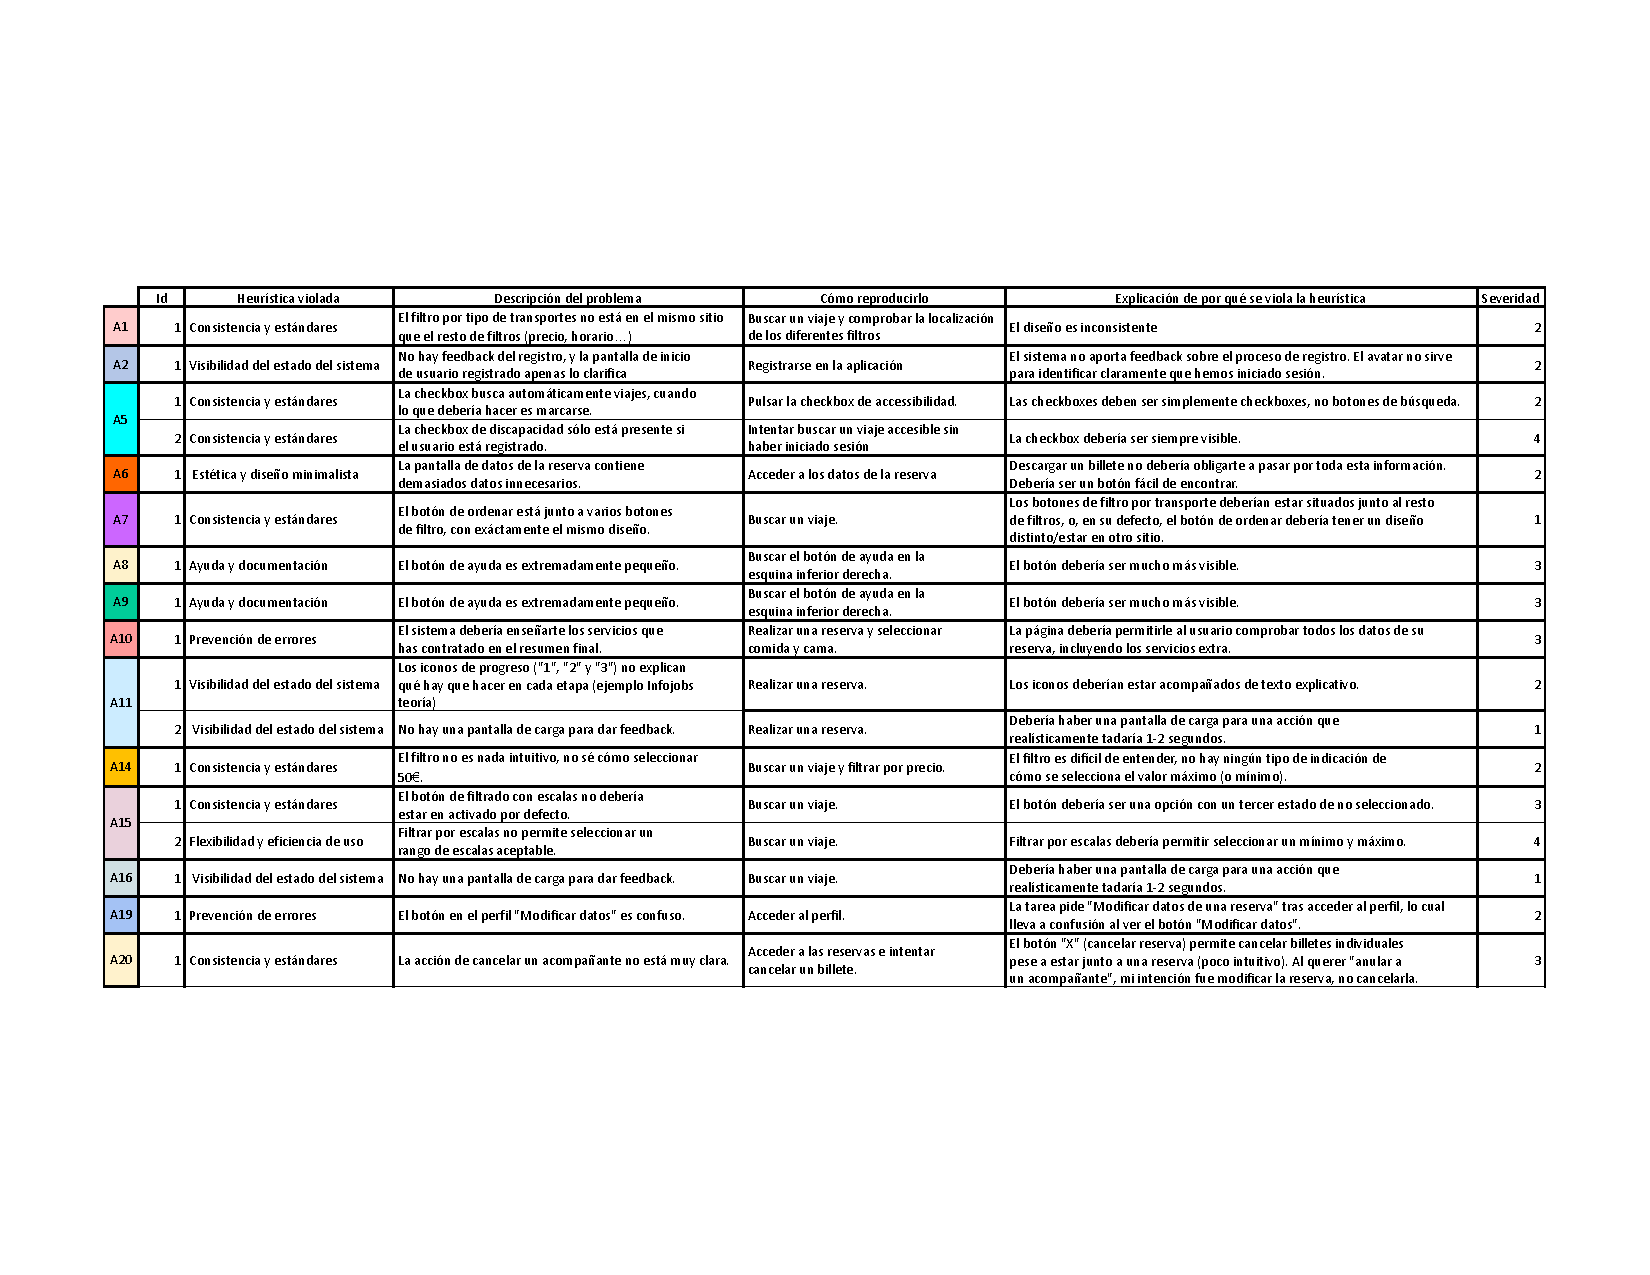
\includegraphics[angle=270,width=1.\textwidth]{Imagenes/Hito6/Evaluación Sesión 1.pdf}
    \caption{Resultado evaluación sesión 1}
    \label{fig:eva-s1}
\end{figure}

\begin{figure}[H]
    \centering
    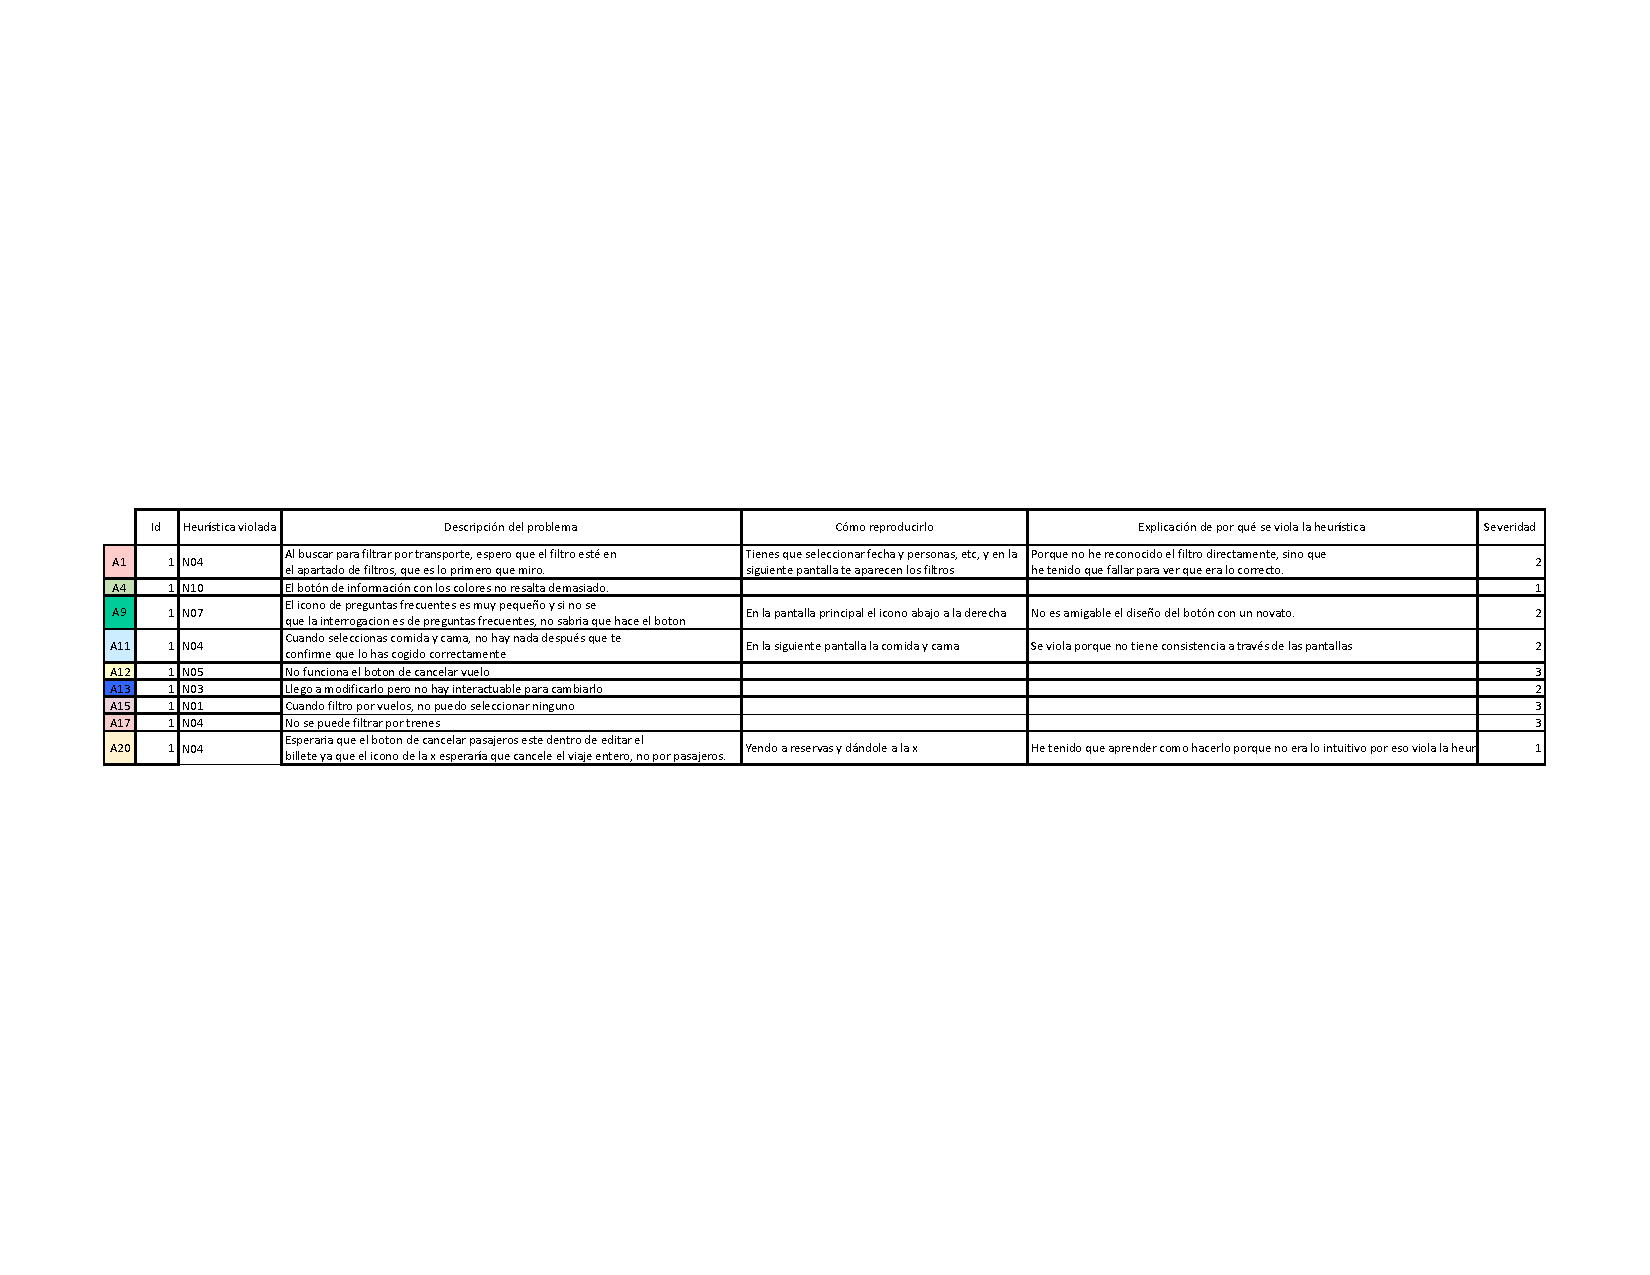
\includegraphics[angle=270,width=1.\textwidth]{Imagenes/Hito6/Evaluación Sesión 2.pdf}
    \caption{Resultado evaluación sesión 2}
    \label{fig:eva-s2}
\end{figure}

\begin{figure}[H]
    \centering
    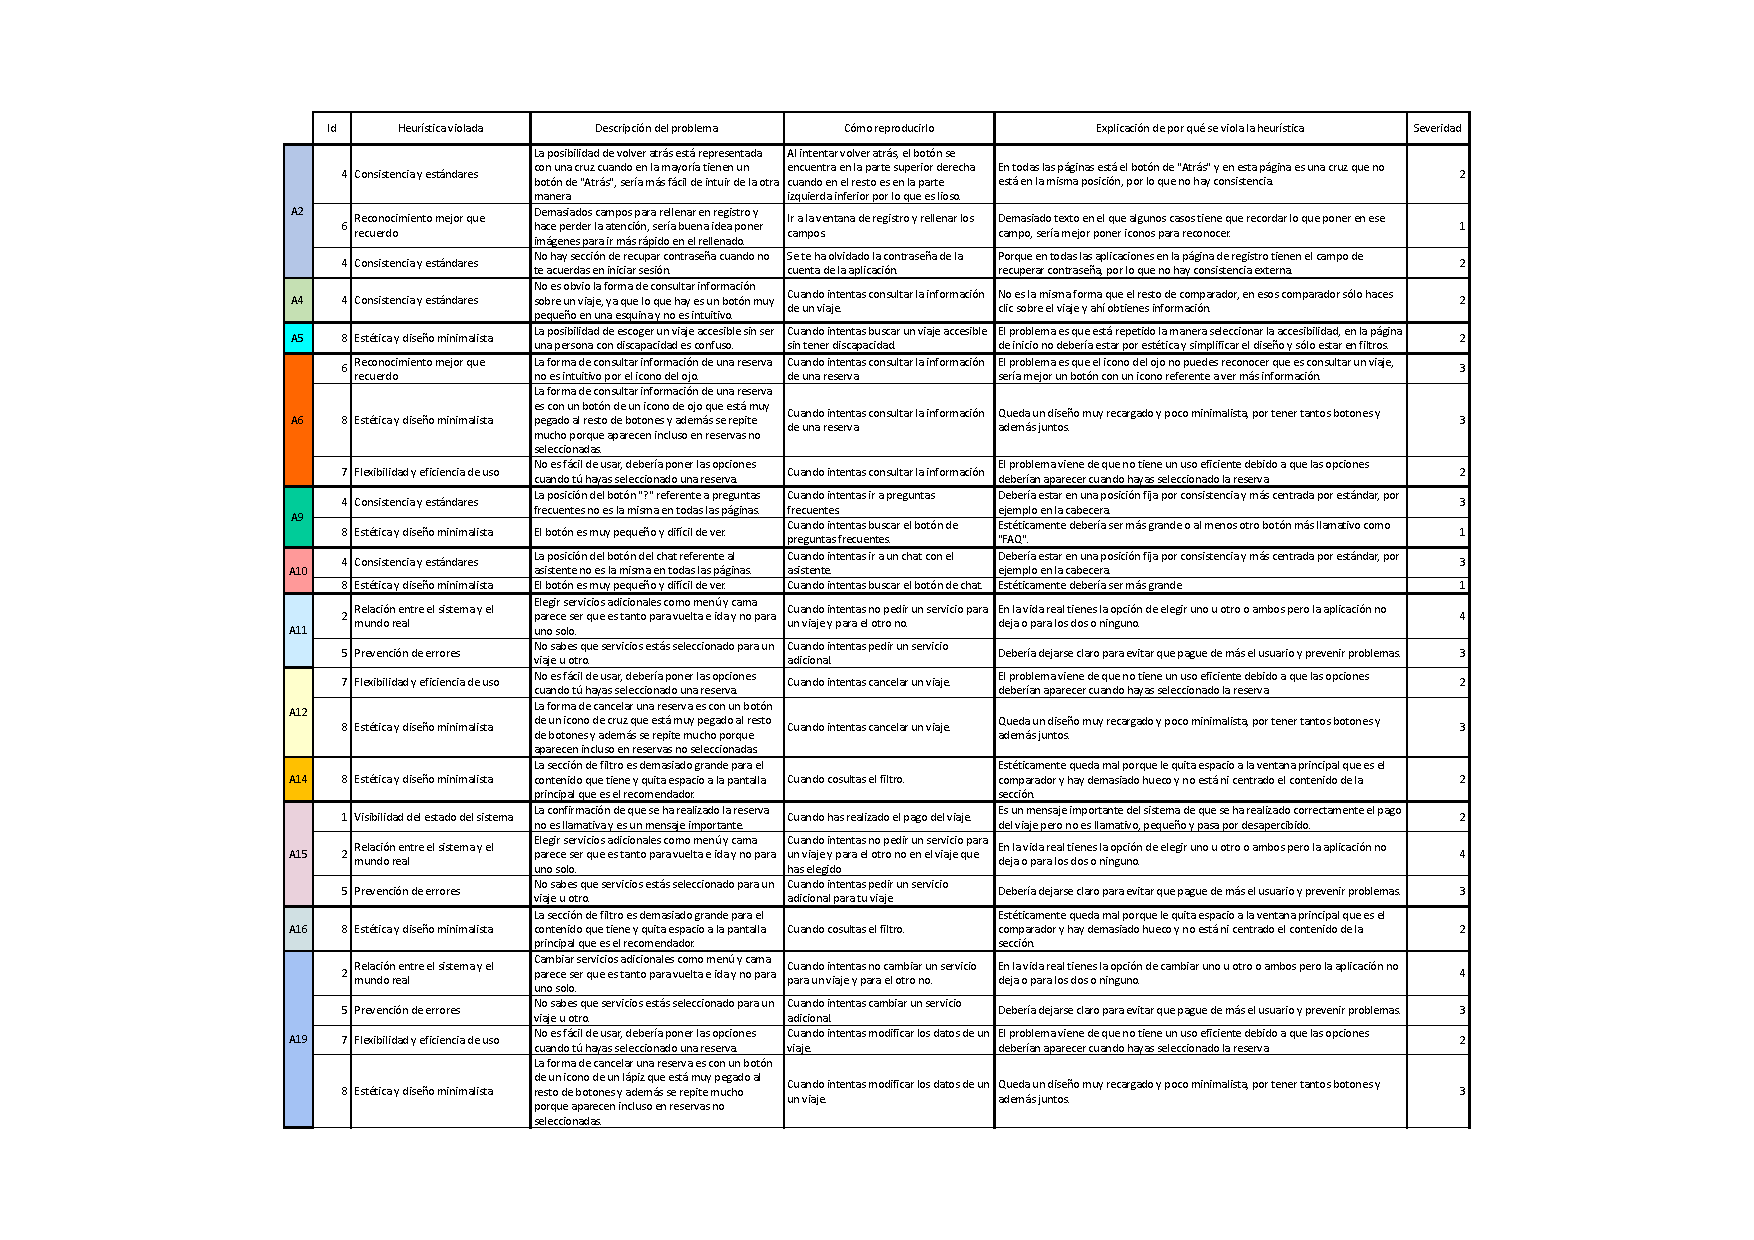
\includegraphics[angle=270,width=1.\textwidth]{Imagenes/Hito6/Evaluación Sesión 3.pdf}
    \caption{Resultado evaluación sesión 3}
    \label{fig:eva-s3}
\end{figure}

\begin{figure}[H]
    \centering
    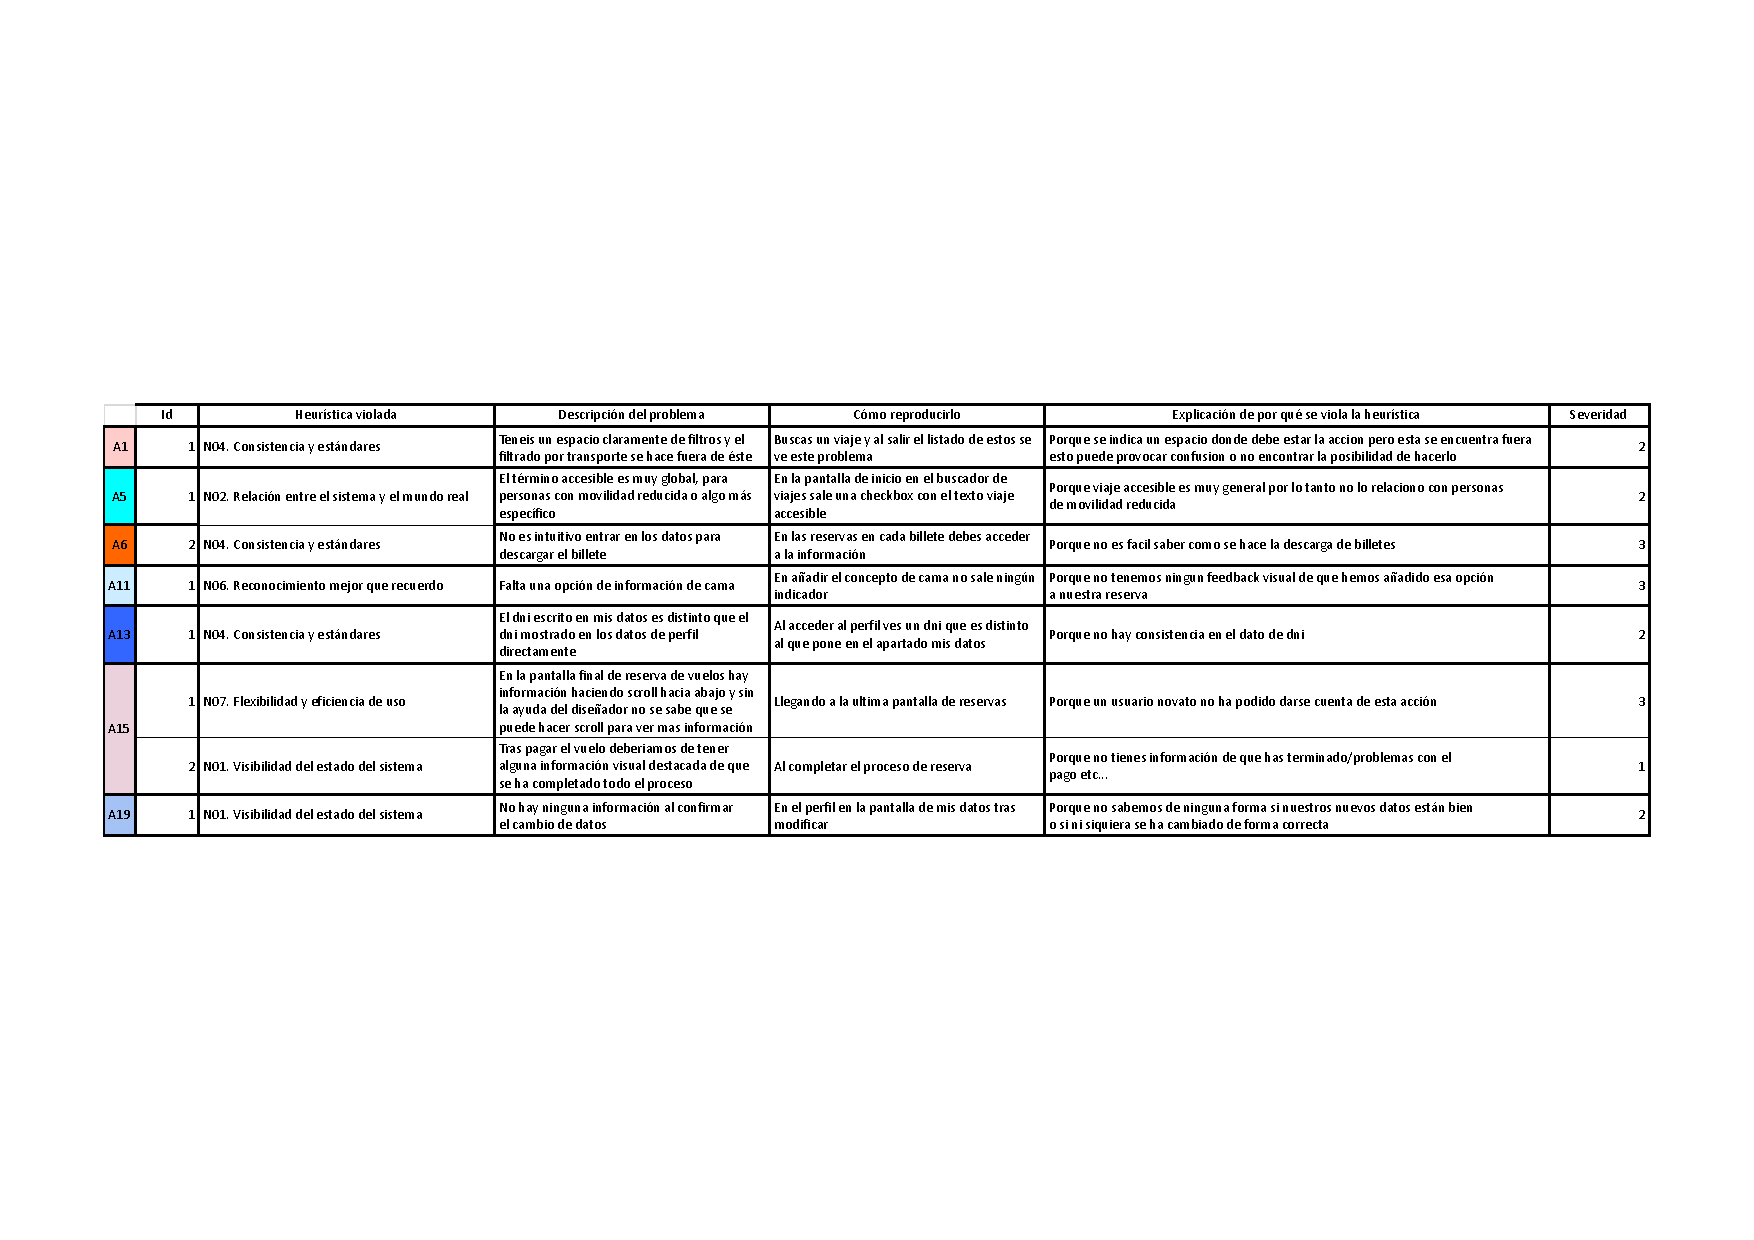
\includegraphics[angle=270,width=1.\textwidth]{Imagenes/Hito6/Evaluación Sesión 4.pdf}
    \caption{Resultado evaluación sesión 4}
    \label{fig:eva-s4}
\end{figure}

\begin{figure}[H]
    \centering
    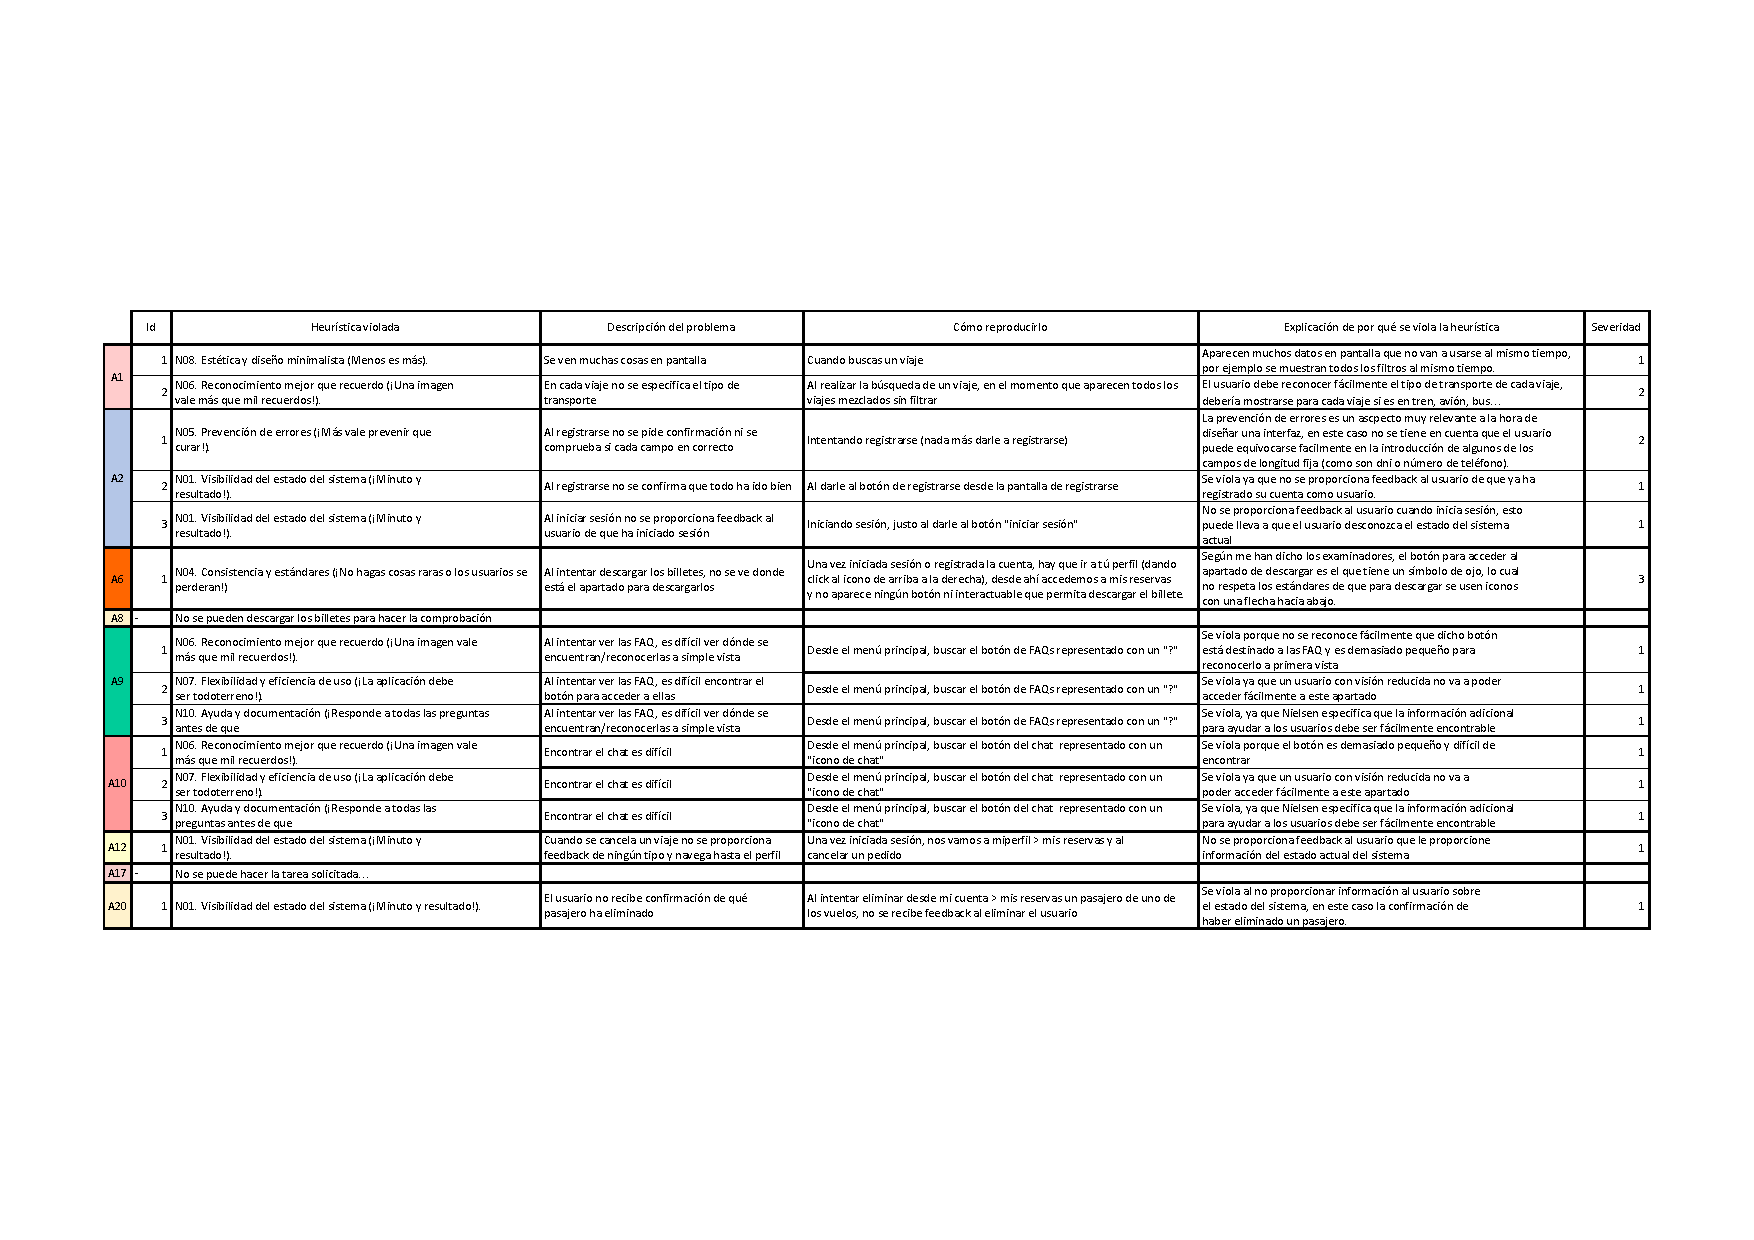
\includegraphics[angle=270,width=1.\textwidth]{Imagenes/Hito6/Evaluación Sesión 5.pdf}
    \caption{Resultado evaluación sesión 5}
    \label{fig:eva-s5}
\end{figure}

\begin{figure}[H]
    \centering
    \includegraphics[angle=270,width=1.\textwidth]{Imagenes/Hito6/Resumen sesiones de evaluación.pdf}
    \caption{Listado del problemas final}
    \label{fig:eva-fin}
\end{figure}

\newpage

\section{Evaluación de las sesiones realizadas para el otro grupo}
En términos generales la evaluación ha sido un éxito. Los expertos en todo momento han mantenido una actitud positiva y de interés a la hora de evaluar la aplicación. 
A pesar de la presencia de inconvenientes con algún experimentador, no ha sido un obstáculo en el ámbito global. Por lo general, la atención de los experimentadores 
también era notable y en consecuencia nuestros expertos han dispuesto todos los fallos de la aplicación en una tabla en la que se distinguen todos los principios 
de heurística que se violan y los motivos. Los experimentadores han dispuesto soluciones de manera constructiva para propiciar el progreso de la aplicación en 
el futuro. Los expertos mantuvieron una mentalidad abierta, comprensiva y preparada para la evaluación. \\

La aplicación gestiona una cafetería, tenía tanto la interfaz del cliente como la del trabajador de la cafetería. Se trataba de un prototipo con un objetivo claro 
y sencillo aunque algunas veces poco intuitivo. En un inicio se les entregó una guía impresa a los expertos para que pudieran evaluar correctamente la aplicación. 
La información y los pasos a seguir eran claros y precisos. Esta guía contaba con una introducción para ayudar al experto a ponerse en contexto, los pasos a seguir 
y por último, los principios heurísticos de Larry Constantine con los que había que trabajar para sacar los fallos. Consideramos que los principios heurísticos que 
nos proporcionaron no eran los adecuados, los expertos averiguaron errores de aplicación y algunos resultaron difíciles de encapsular en los principios de 
Larry Constantine. Creemos que existen otras gamas de principios a seguir más completas y adecuadas a la aplicación que facilitan la atribución de errores a 
principios heurísticos más fácilmente. \\ 

El listado de tareas proporcionado por los experimentadores abordaba la totalidad de la aplicación, por este motivo los expertos fueron capaces de analizar con éxito 
la aplicación. Se ha ido paso a paso y preguntando a los experimentadores todas las dudas que surgían por parte de los expertos. Ahora realizaremos un breve análisis 
de la experiencia de cada experto individualmente.

\subsection{Evaluación Javier}
Javier ha seguido cada uno de los pasos indicados por el experimentador correspondiente. Resaltar que el experimentador no estaba por la labor, estaba poco 
receptivo, a la defensiva y poco atento a las preguntas que realizaba Javier. Por ello, en varias ocasiones, Javier ha tenido que consultar a otros experimentadores 
para poder evaluar de manera correcta la aplicación. El trabajo de Javier ha sido exitoso y ha realizado un análisis de errores de forma constructiva para el 
progreso de la aplicación. Se indicó claramente qué problemas tenía la aplicación, qué principios de la heurística indicada se violaban, cómo abordar los problemas 
y la severidad de los mismos.

\subsection{Evaluación María}
María ha realizado la evaluación siguiendo los pasos indicados por el experimentador del grupo. Se le ha entregado la guía descrita previamente que contaba con 
una explicación contextual de la aplicación y de la dinámica de la evaluación, otra con las acciones a analizar y una última con los principios heurísticos que han 
usado (Larry Constantine). La evaluación ha sido exitosa, se ha analizado cada acción indicando las violaciones de los principios heurísticos encontradas. 
Esta información se ha incluido en una tabla en la que detalladamente se ha explicado el problema encontrado y el principio heurístico violado, con el nivel de
gravedad y las posibles soluciones. El experimentador se ha mostrado muy amable y proactivo en todo momento.

\subsection{Evaluación Daniel}
Daniel ha evaluado la aplicación del grupo 6 siguiendo las acciones dadas por el experimentador. Antes de empezar la evaluación, se han entregado unas hojas que 
contenían la guía de instrucciones, una introducción de la aplicación, y los principios heurísticos a seguir, en el caso del grupo 6, los principios usados han sido 
los de Larry Constantine, como hemos mencionado anteriormente. Después de completar las acciones dadas por el experimentador, y teniendo mayor conocimiento sobre 
la aplicación. Se han evaluado y categorizados los errores encontrados, siguiendo los principios heurísticos proporcionados por el experimentador.

\subsection{Evaluación Pablo}
Pablo ha realizado y al llegar al puesto para realizar dicha evaluación ha sido atendido por un experimentador el cual le ha otorgado la documentación necesaria para 
entender el prototipo y para poder desarrollar las tareas descritas. El material presentado ofrecía información sobre los principios de diseño que se iban a utilizar
para poder evaluar el prototipo: Principios heurísticos de Larry Constantine. \\
En la documentación entregada también se hacía alusión a las tareas que había que realizar como experto. Finalmente se indicaron claramente qué problemas tenía la 
aplicación, qué principios de la heurística indicada se violaban, cómo abordarlos y la severidad de los mismos.

\subsection{Evaluación Rodrigo}
Rodrigo ha realizado la evaluación siguiendo cada uno de los pasos proporcionados por el experimentador, el cual, además de un guión detallado de todas las actividades
de la aplicación aplicables al prototipo, le proporcionó un resumen de los pasos a seguir y de los principios heurísticos empleados por su grupo (Ley de Constantine). \\

El trabajo de evaluación fue notorio, Rodrigo analizó el comportamiento de la aplicación para cada una de las acciones proporcionadas por el experimentador, señalando 
los errores o posibles violaciones de los principios heurísticos. De esta manera y mediante el uso de una tabla excel, fue anotando todos los problemas así como 
las heurísticas violadas, posibles soluciones aplicables y la severidad del error en la aplicación. El experimentador se ha mostrado receptivo y amable solucionando 
cualquier duda que surgía sobre el funcionamiento de la aplicación.

\section{Debriefing}
La última fase del proceso de evaluación es el debriefing. En esta etapa, nos hemos reunido tras las distintas sesiones de evaluación por videollamada el viernes 15 de
Diciembre todos los miembros del grupo para realizar una puesta en común de todos los problemas que habían sido identificados en el listado de las sesiones de evaluación
(figura \ref{fig:eva-fin}). Este listado sirvió como punto de partida, pero el objetivo final de esta reunión era obtener otro listado, en el que nosotros, como diseñadores,
planteásemos una serie de soluciones a los problemas recogidos y en base a estas soluciones, asignarle un coste numérico de 1 a 4 (siendo 1 un coste elevado y 4 un coste
liviano). \\

Esta reunión tuvo una duración de 1 hora, en la que se comenzó realizando una breve lectura de los problemas, revisando previo al debriefing si se encontraba alguna
incoherencia en el listado. Posteriormente, se establecieron las soluciones a cada uno de los problemas y una vez finalizado, se asignaron unos costes. Para finalizar, se
definieron los cambios que se iban a hacer en el prototipo (respetando las prioridades). \\

Tras haber discutido todos los problemas que se encontraban en el listado, plantear las posibles soluciones y asignar un coste a estas soluciones, el siguiente paso seguido
ha sido obtener la prioridad con la que deben de ser solventados estos problemas, siendo los primeros aquellos con una prioridad más elevada. Para poder obtener la prioridad,
han de multiplicarse los valores de la severidad (promedio de los valores proporcionados por los expertos del grupo anterior) y el coste (asignado por nosotros en esta reunión
tras estimar la posible solución). \\

Este nuevo listado (ver figura \ref{fig:list-prob-sol}) va a mantener la esencia del listado final de problemas (los campos del identificador del problema, el título que resuma el problema, la descripción del problema,
la heurística que viola, cómo puede reproducirse y el cálculo de la severidad en función de los valores otorgados por los expertos del grupo 6). A ello hemos añadido una nueva columna
en la que se describe una posible solución al problema (para poder aplicarla en el prototipo), otra para estimar el valor del coste de la solución y por último una para poder
realizar el cálculo de la prioridad. \\

En la siguiente sección, el objetivo es tomar este listado final de problemas, soluciones y prioridades y en el orden establecido por las prioridades, y realizar los cambios pertinentes sobre
el prototipo, siempre respetando las prioridades establecidas, ya que nos van a indicar la necesidad con la que tiene que corregirse este problema sobre el prototipo.
\begin{figure}[H]
    \centering
    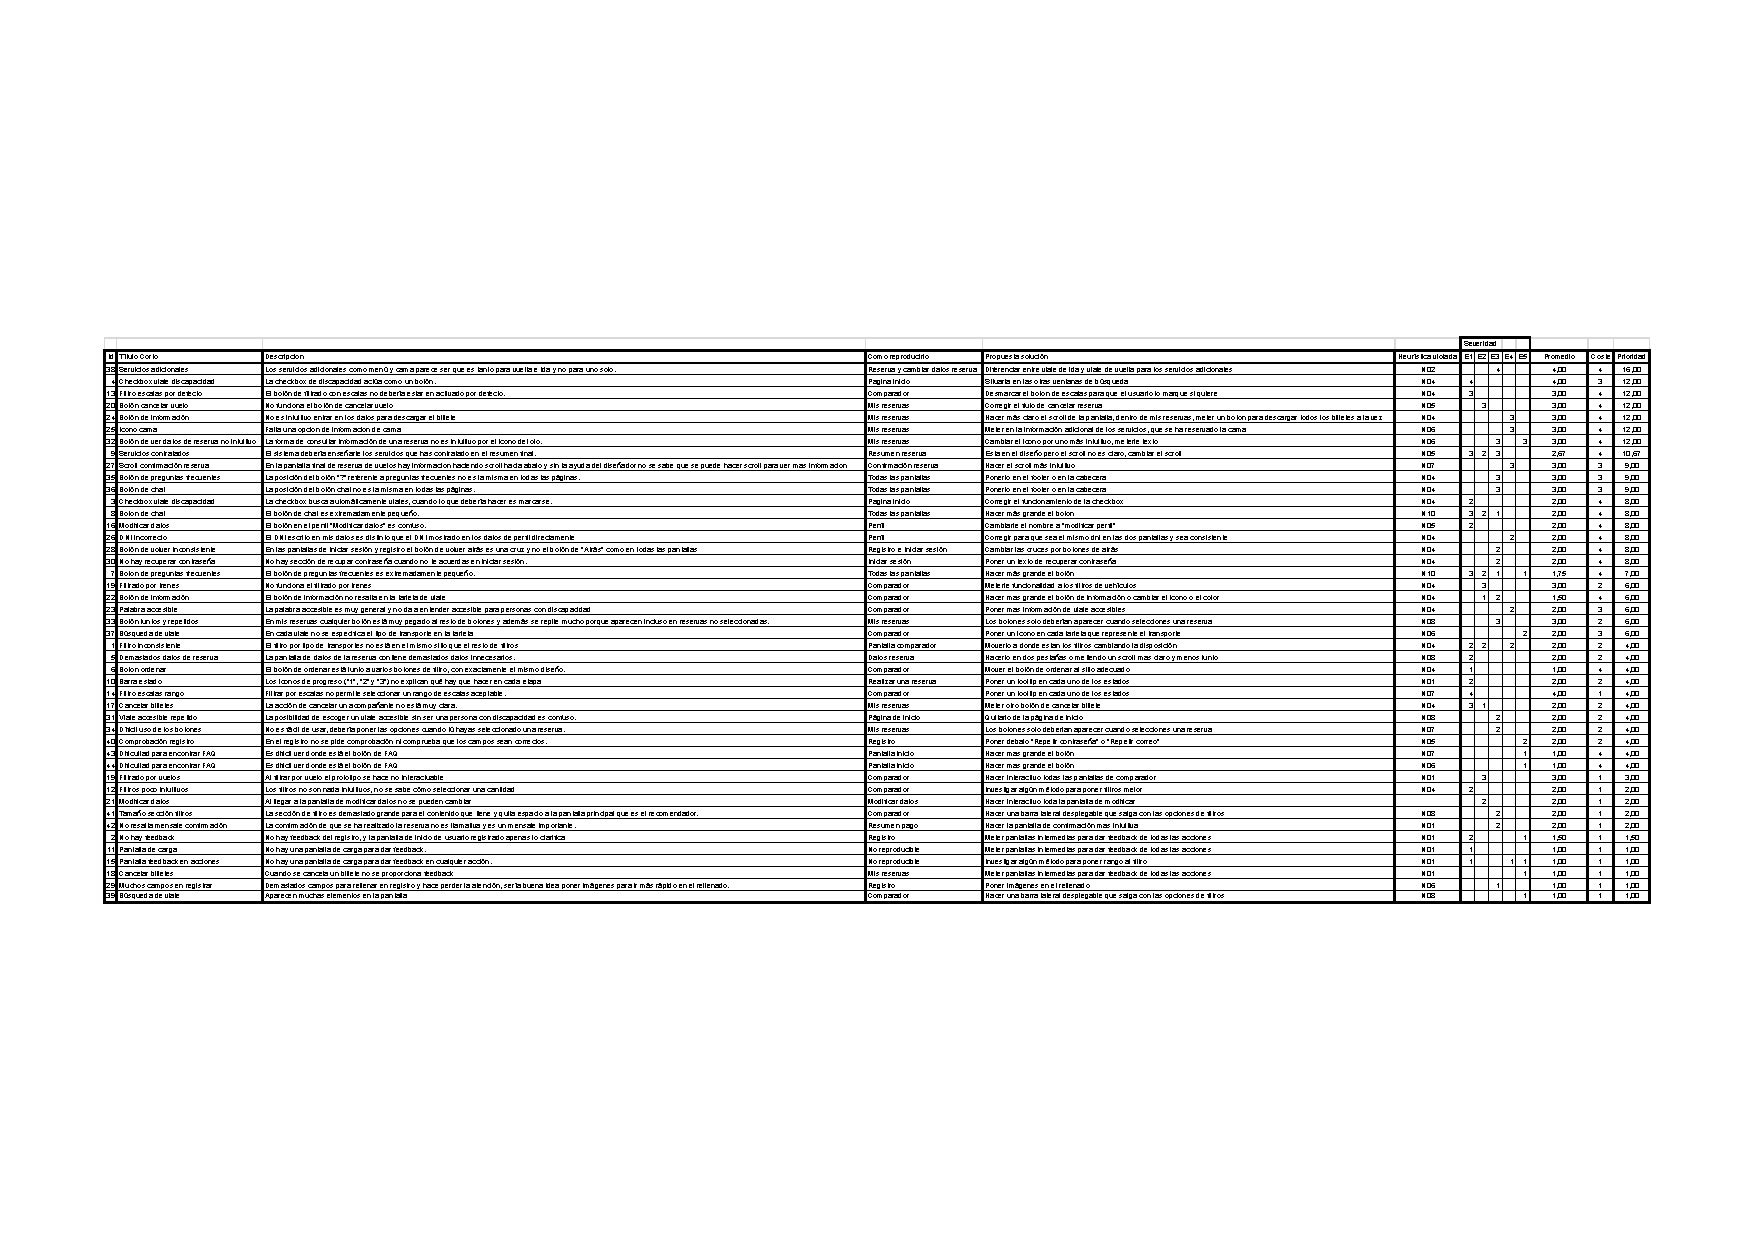
\includegraphics[angle=270,width=1.\textwidth]{Imagenes/Hito6/Lista final de problemas, soluciones y prioridades.pdf}
    \caption{Listado final de problemas y soluciones}
    \label{fig:list-prob-sol}
\end{figure}

\section{Prototipo mejorado}
Por último, una vez obtenido el listado completo de todos los problemas y soluciones, ordenados por la prioridad con la que debían de ser tratados, hemos seleccionado
una serie de estos problemas (ordenados por prioridad) para poder solucionarlos en nuestro prototipo en \href{https://www.figma.com/file/YGz2UUMhvxNOTCHhu1TZle/Just-Travel-It?type=design&node-id=561%3A4382&mode=design&t=TUpWh6Kqo4yieX47-1}{Figma}.
Vamos estos problemas en detalle:
\begin{itemize}
    \item \textbf{Servicios Adicionales} $\rightarrow$ los servicios adicionales de la reserva (como el menú y la cama) no se encuentran diferenciadas entre ida y vuelta. La solución planteada consiste en diferenciar entre ida y vuelta a la hora de seleccionar los servicios.
    \item \textbf{Checkbox viaje discapacidad} $\rightarrow$ la checkbox de discapacidad sólo está presente si el usuario está registrado. La solución 
    \item \textbf{Filtro escalas por defecto} $\rightarrow$ el botón de filtro por escalas se encuentra activado por defecto. La solución es desmarcarlo para que el usuario pueda seleccionarlo cuando desee.
    \item \textbf{Botón cancelar vuelo} $\rightarrow$ tiene un problema de funcionamiento que se soluciona con una corrección del flujo.
    \item \textbf{Botón de información} $\rightarrow$ existe un problema al descargar los billetes, ya que la pantalla en la que se incluyen no tiene un scroll claro, por lo que se ha intentado hacerlo más acorde al principio de cierre.
    \item \textbf{Icono cama} $\rightarrow$ en los servicios contratados no se encuentra la cama anotada si se ha seleccionado el servicio, por lo que ha de añadirse en caso de que se seleccione.
    \item \textbf{Botón de ver datos de reserva no intuitivo} $\rightarrow$ el botón de poder consultar los datos de la reserva no es claro (el icono no es representativo), por lo que ha de cambiarse por otro (se ha optado por una mano seleccionando un ticket).
    \item \textbf{Servicios contratados} $\rightarrow$ el sistema no te muestra los servicios contratados al confirmar la reserva, pero no es cierto, ya que sí se encuentra, pero al no ser claro el scroll se ha optado por hacer algo más claro para evitar confundir a los usuarios.
    \item \textbf{Scroll confirmación reserva} $\rightarrow$ al igual que en el caso anterior, el scroll no es intuitivo, por lo que la solución ha sido hacerlo más claro (aplicando el principio de cierre).
    \item \textbf{Botón de preguntas frecuentes} $\rightarrow$ la posición de este botón no es la misma en todas las pantallas, por lo que se ha establecido una altura fija a la que se va a encontrar y ponerla así en todas las ventanas que lo tengan.
    \item \textbf{Botón de chat} $\rightarrow$ el botón del chat es demasiado pequeño, pudiendo pasar desapercibido por parte de los usuarios, por lo que es necesario ampliar su tamaño.
    \item \textbf{Checkbox viaje discapacidad} $\rightarrow$ uno de los problemas al realizar una búsqueda de viajes accesibles es que al seleccionar la checkbox ya te lleva a la página de viajes accesibles, por lo que ha tenido que modificarse el flujo para hacer búsquedas en función del estado de la checkbox.
    \item \textbf{Botón de chat} $\rightarrow$ el tamaño del botón del chat es demasiado pequeño, por lo que al igual que en el caso de las preguntas frecuentes, puede pasar desapercibido para los usuarios. Es por ello que se ha tenido que aumentar el tamaño de este botón.
    \item \textbf{Modificar datos} $\rightarrow$ el nombre del botón de Modificar Datos (referente a los datos del perfil) es ambiguo, por lo que se ha cambiado a Modificar Perfil para evitar este problema.
    \item \textbf{DNI incorrecto} $\rightarrow$ existe un problema de coherencia, en el que el DNI mostrado en los datos es distinto del DNI del perfil, por lo que se ha corregido este fallo haciendo que en ambos casos sea el mismo.
    \item \textbf{Botón de volver inconsistente} $\rightarrow$ en las pantallas de inicio de sesión y registrarse existe un problema de coherencia en el que el botón de retroceder, en vez de ser un botón con el texto Atrás es una X. Se ha tenido que modificar para corregir este fallo.
    \item \textbf{No hay recuperar contraseña} $\rightarrow$ existe un problema a la hora de iniciar sesión, ya que no se puede brindar al usuario la opción de recuperar la contraseña en caso de que la haya perdido.
    \item \textbf{Botón de preguntas frecuentes} $\rightarrow$ al igual que ocurre con el soporte, el botón de las preguntas frecuentes también es muy poco intuitivo y puede no ser detectado por los usuarios.
\end{itemize}

Estos problemas se han solventado en este orden y con las soluciones que se han planteado, de modo que el prototipo ya se encuentra preparado para la evaluación con los
usuarios finales que va a ser realizada en el siguiente hito, reduciendo así la cantidad de problemas que han de detectarse.
